%!TEX root = ../dissertation.tex

\hypertarget{(chap:capitolo3)}{}
\chapter{Inquadramento delle attività di stage}
\section{Il progetto aziendale}
Per riuscire ad inquadrare al meglio lo scopo del progetto di stage è importante capire a fondo il progetto generale che l'azienda porta avanti da ormai alcuni anni, poiché essi sono tra loro intrinsecamente legati. Il progetto generale mira a fornire un prodotto che possa far progredire il mercato del trasporto attraverso la digitalizzazione dello stesso, questo attraverso il superamento dei vecchi gestionali, utilizzati concretamente solo per la fatturazione, e l'introduzione di una piattaforma web attraverso cui gestire ogni passaggio nel rapporto cliente-operatore.\\
Il software permette di gestire la flotta di mezzi e organizzare gli ordini di carico-scarico commissionati dai clienti, questa organizzazione può essere fatta manualmente da un operatore esperto oppure affidandosi ad algoritmi che organizzino gli ordini utilizzando i camion disponibili nel miglior modo possibile.\\
Il sistema dispone di un algoritmo per il \glo{vehicle routing}, su cui si può dire faccia capo l'intero progetto, questo si occupa di ottimizzare i viaggi dei camionisti tenendo conto di un numero incredibile di variabili, questo algoritmo ha subito diversi rilasci in un'ottica di miglioramento continuo, per renderlo sempre più efficiente, versatile e preciso.\\
In questo contesto avere un'euristica che fornisca la valutazione approssimativa dello spazio occupato da un certo numero di merci è molto importante, questo perché è necessario sapere quanti mezzi siano necessari per trasportare le merci richieste e quanto spazio sia ancora disponibile per ordini futuri.

\section{Il progetto di stage}
Il progetto di stage dopo l'evento \glo{StageIt} ed alcune riunione presso l'azienda è stato studiato dettagliatamente e riportato nel documento piano di lavoro, nello stesso sono riportati gli obiettivi e la pianificazione delle attività.\\
L'importanza di ottenere una valutazione reale dello spazio occupato da un certo numero di oggetti è fondamentale, per fare ciò lo stage prevede la realizzazione di diversi modelli, lo sviluppo di tali modelli sarà incrementale in quanto ciascun modello eredita quanto sviluppato nel precedente.\\
Ogni modello per definizione permetterà di individuare la disposizione ottima dell'\glo{istanza} corrente, questa potrà poi essere confrontata con quella fornita dall'euristica. Dal confronto potremo individuare informazioni utili che permettano di valutare oggettivamente la bontà delle soluzioni fornite dall'euristica, allo scopo di capire se con il passare delle versioni rilasciate l'euristica stia migliorando e di quanto rispetto alle versioni passate.

\section{Astrazione del problema}
Una possibile astrazione del problema è considerare il container e le merci come se fossero parallelepipedi.\\
Questa astrazione è necessaria per poter approssimare il tutto come richiesto dal \textit{Bin Packing Problem}, problema su cui si è studiato e discusso molto in ambito accademico portando alla realizzazione di algoritmi esatti ed euristiche.\\
Si consideri un insieme I = \{1,...,n\} di oggetti aventi dimensioni $w_{i}$, $d_{i}$ e $h_{i}$ con i $\in$ I, un insieme J = \{1,...,m\} di contenitori di uguale dimensione W, D e H, ogni oggetto $i \in I$ ha la possibilità di essere ruotato di 90° rispetto la propria base e si da per ipotesi che $w_{i} \leq W$, $d_{i} \leq D$ e $h_{i} \leq H$, inoltre è possibile che gli oggetti vengano sovrapposti, l'obiettivo è di utilizzare il minor numero di contenitori J che riescano a contenere tutti gli oggetti dell'insieme I.
\begin{figure}[H]
	\begin{center} 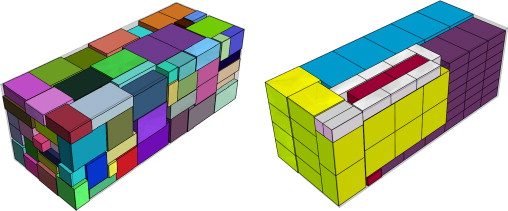
\includegraphics[scale=0.8]{figures/bin_packing}
		\caption[Contenitori Bin Packing]{Due contenitori completamente pieni}  
	\end{center}
\end{figure}

\section{Variante del Bin Packing}
Una variante del problema del Bin Packing, il più famoso di una lunga serie di problemi di disposizione di oggetti in contenitori, è lo \textit{Strip Packing Problem}, le differenze principali dal precedente possono essere individuate di seguito:
\begin{itemize}
	\item \textbf{Numero di contenitori}: viene utilizzato un singolo contenitore;
	\item \textbf{profondità}: la profondità del contenitore è infinita;
	\item \textbf{Oggetti}: come obiettivo si quello di occupare minor spazio lineare possibile rispetto la profondità del contenitore.
\end{itemize}
